\documentclass[20pt]{beamer}
\usepackage{array} % Used for > in Resources table

% Colours come from colour brewer
\usepackage{xcolor}
\definecolor{b-blue}{HTML}{6baed6}
\definecolor{b-darkgrey}{HTML}{2D2D2D}
\definecolor{b-grey}{HTML}{969696}
\definecolor{b-purple}{HTML}{9e9ac8}
\definecolor{b-green}{HTML}{74c476}
\definecolor{b-pink}{HTML}{e377c2}
\definecolor{b-orange}{HTML}{FD8D3C}

\usepackage{relsize}

\usepackage{fontspec}
\defaultfontfeatures{Mapping=tex-text} % enable -- / --- / `` / ''
\setsansfont[ItalicFont={* Light},BoldItalicFont={* ExtraLight}]{Yanone Kaffeesatz}
\setmonofont[Scale=0.75]{Bitstream Vera Sans Mono}

% Neutralise underscores, since we don't use them apart for in URLs
\catcode`_=12
\begingroup\lccode`~=`_\lowercase{\endgroup\let~\sb}
\mathcode`_="8000



% Enforce colours and styles for beamer:
\setbeamercolor*{palette primary}{fg=white,bg=b-darkgrey}
\setbeamercolor*{titlelike}{parent=palette primary}
\setbeamercolor*{normal text}{parent=palette primary}
\setbeamercolor*{itemize}{parent=palette primary}
\color{white}

\setbeamertemplate{navigation symbols}{}
\setbeamercolor{itemize/enumerate body}{fg=white}
\setbeamercolor{enumerate item}{fg=white}
\setbeamertemplate{itemize item}{\raisebox{.33ex}{\footnotesize\color{white}$\blacktriangleright$}}

\usepackage{tikz}
\usetikzlibrary{positioning}
\usetikzlibrary{shapes.geometric}
\usetikzlibrary{calc}
% Useful for pictures.
\tikzstyle{nopadding} = [inner sep=0cm]
\tikzstyle{attribution} = [fill=b-darkgrey, anchor=south,
outer sep=0, inner sep=.1ex, font=\relsize{-6}\it,
minimum width=\paperwidth, text width=.95\paperwidth]

\newcommand{\hero}[1]{%
  \begin{tikzpicture}[remember picture, overlay]%
  \node[anchor=west,align=left,font=\Huge\bfseries] (A) at ($(current page.west) + (0.05\paperwidth, .17\paperheight)$) {%
    #1
  };
\end{tikzpicture}}

\newcommand{\herohigh}[1]{%
  \begin{tikzpicture}[remember picture, overlay]%
  \node[anchor=west,align=left,font=\Huge\bfseries] (A) at ($(current page.west) + (0.05\paperwidth, .25\paperheight)$) {%
    #1
  };
\end{tikzpicture}}

\newcommand{\minionhigh}[1]{%
  \begin{tikzpicture}[remember picture, overlay]%
  \node[anchor=west,align=left,font=\Large\bfseries] (A) at ($(current page.west) + (0.05\paperwidth, .25\paperheight)$) {%
    #1
  };
\end{tikzpicture}}

\newcommand{\upperhalf}[1]{%
  \begin{tikzpicture}[remember picture, overlay]%
    \node[anchor=west,font=\normalsize, align=left] at
    ($(current page.west) + (0.05\paperwidth, .25\paperheight)$) {%
      #1
    };
  \end{tikzpicture}
}

\newcommand{\lowerhalf}[1]{%
  \begin{tikzpicture}[remember picture, overlay]%
    \node[anchor=west,font=\normalsize, align=left] at
    ($(current page.west) + (0.05\paperwidth, -.25\paperheight)$) {%
      #1
    };
  \end{tikzpicture}
}

\newcommand{\bottomhalf}[1]{%
  \begin{tikzpicture}[remember picture, overlay]%
    \node[anchor=south west,font=\normalsize, align=left] at
    ($(current page.south west) + (0.05\paperwidth, 0)$) {%
      #1
    };
  \end{tikzpicture}
}

\newcommand{\inthemiddle}[1]{%
  \begin{tikzpicture}[remember picture, overlay]%
    \node at (current page.center) {%
      #1
    };
  \end{tikzpicture}
}

\newcommand{\bottomleft}[1]{%
  \begin{tikzpicture}[remember picture, overlay]%
    \node[anchor=south west, align=left,font=\footnotesize] at (current page.south west) {%
      #1
    };
  \end{tikzpicture}
}

\newcommand{\bottomright}[1]{%
  \begin{tikzpicture}[remember picture, overlay]%
    \node[anchor=south east, align=right,font=\footnotesize] at (current page.south east) {%
      #1
    };
  \end{tikzpicture}
}

\newcommand{\bottomhanging}[1]{%
  \begin{tikzpicture}[remember picture, overlay]%
    \node[anchor=north] at
    ($(current page.center) + (0, .17\paperheight)$) {
      #1
    };
  \end{tikzpicture}
}

\newcommand{\bottomhangingborder}[1]{%
  \begin{tikzpicture}[remember picture, overlay]%
    \node[anchor=north, fill=white, rounded corners,
  draw=b-orange, line width=2pt] at
    ($(current page.center) + (0, .17\paperheight)$) {
      #1
    };
  \end{tikzpicture}
}

\newcommand{\bottomhangingleft}[1]{%
  \begin{tikzpicture}[remember picture, overlay]%
    \node[anchor=north west,align=left] at
    ($(current page.west) + (0.05\paperwidth, .17\paperheight)$) {
      #1
    };
  \end{tikzpicture}
}

\usepackage{modules/tex/fontawesome}

\def\twitter{{\FA \faTwitter}}
\def\heart{{\FA \faHeart}}
\def\tickmark{{\FA \faCheck}}
\def\rarrow{{\FA \relsize{-1}{\faArrowRight}}}

\def\imagetop#1{\vtop{\null\hbox{#1}}}

\newcommand{\hrefp}[2]{\href{#1://#2}{#2}}
\newcommand{\twitterhandle}[1]{\href{https://twitter.com/#1}{\twitter #1}}
\newcommand{\twitterhandlesm}[1]{\relsize{-1}{\color{b-grey}\href{https://twitter.com/#1}{@#1}}}

\begin{document}

\begin{frame}
  \begin{tikzpicture}[remember picture, overlay]
    \node (A) at ($(current page.center) + (0, .17\paperheight)$) {
      \resizebox{.9\paperwidth}{!}{%
        \color{b-blue}\bf The challenge of combining 176 x \#otherpeoplesdata to create}
    };
    \node[anchor=north] at (A.south) {
      \resizebox{.9\paperwidth}{!}{%
        \color{b-green}the Biomass And Allometry Database (BAAD)}
    };
    \color{white}
    \node[anchor=south west] (B) at
    ($(current page.south west) + (0.05\paperwidth, 0.05\paperwidth)$) {
      \resizebox{.9\paperwidth}{!}{%
      \color{b-grey}\twitterhandle{adaptive\_plant},
       \href{mailto: daniel.falster@mq.edu.au}{{ \FA \faEnvelope} daniel.falster@mq.edu.au}, 
      \href{http://danielfalster.com}{{\FA \faHome} danielfalster.com}
      }
    };
    \node[anchor=south west] at (B.north west) {
      \resizebox{.9\paperwidth}{!}{%
        \color{white} 
        Daniel Falster, Rich FitzJohn, Remko Duursma, Diego Barneche}
    };
 \end{tikzpicture}
\end{frame}

%-----------------------------------
\begin{frame}\frametitle{\color{b-blue} A compilation}

\begin{tikzpicture}[remember picture, overlay]
  \node[anchor = south, align=center, fill=white, rounded corners,
  draw=b-orange, line width=2pt] at ($(current page.south) +(0,1cm)$) {
    \includegraphics<1>[width=0.9\textwidth]{downloads/map.png}
  };
  \end{tikzpicture}
\end{frame}


%-----------------------------------
\begin{frame}\frametitle{\color{b-purple} ... of field data}
\begin{tikzpicture}[remember picture, overlay]
  \node[anchor = south, align=center] at ($(current page.south) +(0,0.25cm)$) {
    \includegraphics<1>[width=0.95\textwidth]{pics/baad/Slide09.jpg}
    \includegraphics<2>[width=0.95\textwidth]{pics/baad/Slide10.jpg}
  };
  \end{tikzpicture}
\end{frame}

%-----------------------------------
\begin{frame}\frametitle{ Why (1): \color{b-blue} We needed data}
\begin{tikzpicture}[remember picture, overlay]
  \node[anchor = north, align=center, fill=white, rounded corners,
  draw=b-orange, line width=2pt] at ($(current page.south) +(0,8cm)$) {
    \includegraphics<1>[width=0.6\textwidth]{figures/tradeoff-Falster2015-2.pdf}
    \includegraphics<2>[width=0.6\textwidth]{figures/tradeoff-Falster2015-3.pdf}
   };
  \end{tikzpicture}
\end{frame}

%-----------------------------------
\begin{frame}\frametitle{\color{b-pink} 61 Variables}
\begin{tikzpicture}[remember picture, overlay]
  \node[anchor = south, align=center, fill=white, rounded corners,
  draw=b-green, line width=2pt] at ($(current page.south) +(1, 0.25cm)$) {
    \includegraphics<1>[width=0.7\textwidth]{figures/baad_variable_count.pdf}
   };
  \end{tikzpicture}
\end{frame}

%-----------------------------------
{\setbeamercolor{background canvas}{bg=black}
\setbeamercolor{frametitle}{bg=black}
\begin{frame}\frametitle{ Why (2):\color{b-blue} Trial new techniques}
\begin{tikzpicture}[remember picture, overlay]
  \node[anchor = north, align=center] at ($(current page.south) +(0,8.5cm)$) {
    \includegraphics[width=0.55\textwidth]{downloads/BTFF15.jpg}
   };
  \end{tikzpicture}
\end{frame}
}
%-----------------------------------


\begin{frame}
  \herohigh{Lots of {\color{b-pink} small data}}
  \bottomhanging{
    
\includegraphics[width=0.9\paperwidth]{pics/baad/Collage}
  }
\end{frame}

\begin{frame}
  \herohigh{{\color{b-blue} \#otherpeoplesdata}}
  \begin{tikzpicture}[remember picture, overlay]
  \node[anchor = south, align=center] at ($(current page.south) +(0, 2cm)$) {
      
\includegraphics[width=.85\paperwidth]{shots/otherpeoplesdata.png}
 };
  \end{tikzpicture}
\end{frame}


\begin{frame}
  \herohigh{\color{b-purple} Script everything}

  \begin{tikzpicture}[remember picture, overlay]%
    \node[anchor=north, align=center] at
    ($(current page.center) + (0, .17\paperheight)$) {
    \includegraphics[width=.95\paperwidth]{snippets/baad_rebuild}};
    
    \node[anchor=north, align=center] at
    ($(current page.center) + (0, -.2\paperheight)$) {
    \only<2>{\normalsize {\FA \faThumbsUp} Easy to modify, transparent, extensible}
    };
  \end{tikzpicture}
\end{frame}


\begin{frame}
  \herohigh{\color{b-pink} Principles}
 
  \begin{tikzpicture}[remember picture, overlay]%
    \node [anchor=north, align=left] at
    ($(current page.center) + (0, .17\paperheight)$) {%
      \begin{tabular}{c l}
        & Pipeline for processing and review\\
        & Don't modify raw data files \\
        & Encode meta-data as data \\
        & Version control \\
      \end{tabular}
  };
  \end{tikzpicture}
\end{frame}


\begin{frame}
  \herohigh{\color{b-purple} Pipeline}
  \bottomhangingborder{
    \includegraphics[width=.75\paperwidth]{downloads/pipeline.png}
  }
\end{frame}

\begin{frame}
  \minionhigh{\color{b-purple} Encode meta-data as data}
  \bottomhanging{
    \includegraphics[width=.95\paperwidth]{snippets/baad_dataMatch}
  }
\end{frame}

\begin{frame}
  \herohigh{\color{b-pink} Review}
  \bottomhangingborder{
    \includegraphics[width=.75\paperwidth]{downloads/data_review_error.png}
  }
\end{frame}

\begin{frame}
  \herohigh{\color{b-purple}  Collaborate}%
  \lowerhalf{
    \LARGE {\color{white} R + {\color{b-purple} git} +
          {\color{b-orange}GitHub} =} {\color{b-pink}\heart}%
  }
\end{frame}

\begin{frame}
  \only<1>{\minionhigh{Work on same code base\phantom{g}}}%
  \only<2>{\minionhigh{See what changed}}%
  \bottomhanging{%
    \includegraphics<1>[width=0.9\paperwidth]{shots/version_control_collaboration}%
    \includegraphics<2>[width=0.9\paperwidth]{shots/version_control_changes}
    }
\end{frame}


\begin{frame}
  \minionhigh{\LARGE{\color{b-pink} CI} {\color{white} = }\color{b-blue}Continuous Integration}
  \lowerhalf{
    \begin{minipage}{\textwidth}
      \begin{enumerate}
      \item Commit changes
      \item Push to GitHub
      \item Get an email if something breaks
      \end{enumerate}
    \end{minipage}
  }
  \note{}
\end{frame}

\begin{frame}
  \minionhigh{%
    \only<1>{Runs on virtual machine\ldots}}
  \bottomhanging{%
    \includegraphics<1>[width=\paperwidth]{shots/travis_spinup}%
  }
\end{frame}

\begin{frame}
  \minionhigh{Set and forget -- never gets bored}
  \bottomhanging{
    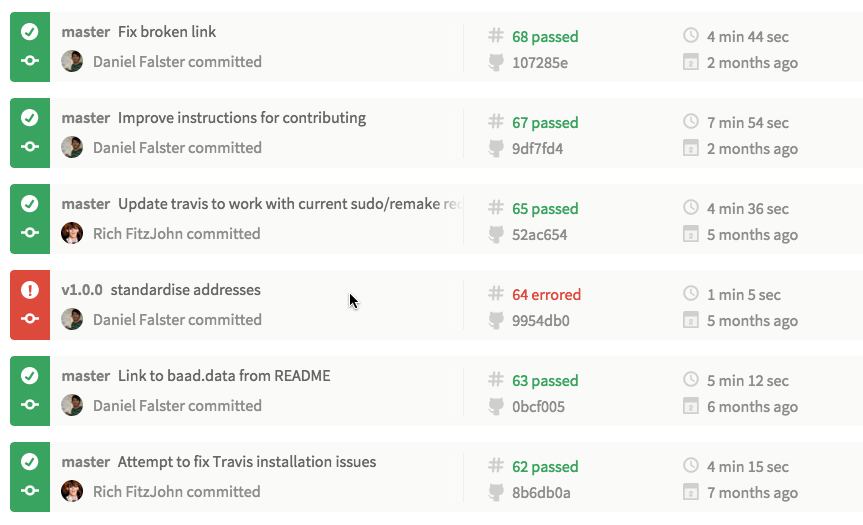
\includegraphics[width=0.65\paperwidth]{shots/travis_builds}%
  }
  \bottomleft{\href{https://travis-ci.org/dfalster/baad/builds}{travis-ci.org/dfalster/baad/builds}}
\end{frame}

\begin{frame}
  \herohigh{\color{b-purple} Entirely open}
  \bottomhanging{
    \includegraphics<1>[width=.85\paperwidth]{pics/baad/F2015.png}
    \includegraphics<2>[width=.95\paperwidth]{snippets/baad_package}
  }
\end{frame}

\begin{frame}
  \herohigh{\color{b-purple} Started open}
    \begin{tikzpicture}[remember picture, overlay]%
    \node[anchor=north west, align=left, text width=12cm] at
    ($(current page.west) + (0.05\paperwidth, 0.05\paperheight)$) {
      \footnotesize
        {\color{b-blue} Daniel:} {\color{white}Would you like to co-author a data paper in Ecology? }\\
        
        {\color{b-pink} Yes {\FA \faArrowRight}}  {\color{white}Great, tell us what you've got.} \\
    
        {\color{b-pink} No {\FA \faArrowRight}}  {\color{white} No worries. Get back to us if you change you're mind.}\\
    };
  \end{tikzpicture}
\end{frame}

\begin{frame}
  \herohigh{\color{b-purple} remake}
  \bottomhanging{
    \includegraphics<1>[width=0.8\paperwidth]{shots/remake_diagram}%
    \includegraphics<2>[width=1\paperwidth]{shots/remake_duursma}%
    \includegraphics<3>[width=0.8\paperwidth]{snippets/remake_figures}%
    \includegraphics<4>[width=0.7\paperwidth]{snippets/remake_yaml}%

  }
\end{frame}

\begin{frame}\frametitle{ {\color{b-pink} Thanks to collaborators}}
  
  \begin{tikzpicture}[remember picture, overlay]%
    \node [anchor=north, align=left] at
    ($(current page.center) + (0, .4\paperheight)$) {%
    {\small
      \begin{tabular}{c >{\color{white}}l  c >{\color{white}}l }
        \raisebox{-.03\paperheight}{%
          
\includegraphics[height=.12\paperheight]{pics/people/FitzJohn}}&
        Rich FitzJohn  & 
        \raisebox{-.03\paperheight}{%
          
\includegraphics[height=.12\paperheight]{pics/people/Duursma}}&
        Remko Duursma  \\
        \raisebox{-.03\paperheight}{%
          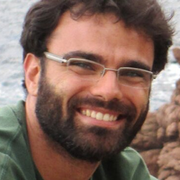
\includegraphics[height=.12\paperheight]{pics/people/Barneche}}&
        Diego Barneche & 
        \raisebox{-.03\paperheight}{%=
          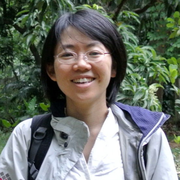
\includegraphics[height=.12\paperheight]{pics/people/Ishihara}}&
        Masae Ishihara \\
     \end{tabular}
      }
  };
  \node [anchor=south, align=left, text width = 12cm] at
    ($(current page.south) + (0, 0.05cm)$) {%
   {\baselineskip=2.5pt\fontsize{9pt}{9pt} \selectfont  \color{white} \\
   {\color{b-blue}Australia:} Angelica V{\aa}rhammar, Michael Aspinwall, Michael Battaglia, James Camac, Steve Hamilton, Lindsay Hutley, Karel Mokany, Anthony O'Grady, Olusegun Osunkoya, David Tissue, Elizabeth Wenk, Richard Williams,Fabiano de Aquino Ximenes \par
   \vspace{1em}
   {\color{b-blue} World:} Masahiro Aiba, Makoto Ando, Niels Anten, Jennifer Baltzer, Christopher Baraloto, John Battles, Ben Bond-Lamberty, Michiel van Breugel,  Yves Claveau, Lluís Coll, Masako Dannoura, Sylvain Delagrange, Jean-Christophe Domec, Farrah Fatemi, Wang Feng, Veronica Gargaglione, Yoshiaki Goto, Akio Hagihara, Jefferson Hall, Degi Harja, Tsutom Hiura, Robert Holdaway,  Tomoaki Ichie, Eric Jokela, Anu Kantola, Jeff Kelly, Tanaka Kenzo, David King, Brian Kloeppel, Takashi Kohyama, Akira Komiyama, Jean-Paul Laclau, Christopher Lusk, Douglas Maguire, Guerric le Maire, Annikki M{\"a}kel{\"a}, Lars Markesteijn, John Marshall, Katherine McCulloh, Itsuo Miyata, Shigeta Mori, Randall Myster, Masahiro Nagano, Shawna Naidu, Yann Nouvellon, Kevin O'Hara, Toshiyuki Ohtsuka, Noriyuki Osada,  Pablo Luis Peri, Any Mary Petritan, Lourens Poorter, Angelika Portsmuth, Catherine Potvin, Johannes Ransijn, Douglas Reid, Sabina Ribeiro, Scott Roberts, Rolando Rodríguez, Angela Salda{\~n}a-Acosta, Ignacio Santa-Regina, Kaichiro Sasa, Galia Selaya, Stephen Sillett, Frank Sterck, Kentaro Takagi, Takeshi Tange, Hiroyuki Tanouchi, Toru Umehara, Hajime Utsugi, Matthew Vadeboncoeur, Fernando Valladares, Petteri Vanninen, Jian Wang, Atsushi Yamaba, Toshihiro Yamada, Takuo Yamakura, Ruth Yanai, Robert York \par
}
   };

  \end{tikzpicture}
\end{frame}

\begin{frame}
  \herohigh{\color{b-blue}Resources}
  \begin{tikzpicture}[remember picture, overlay]%
    \node[anchor=north west,align=left,font=\small] at
    ($(current page.west) + (0.05\paperwidth, .17\paperheight)$) {
      \begin{tabular}{>{\color{white}}r >{\color{b-grey}\footnotesize}l}
      Blog post &
      \hrefp{http}{ropensci.org/blog/2015/06/03/baad/}\\      
      Paper &
      \hrefp{http}{doi.org/10.1890/14-1889.1}\\
      Code &
      \hrefp{https}{github.com/dfalster/baad}\\
      Baad.data&
      \hrefp{https}{github.com/traitecoevo/baad.data}\\
      Remake &
      \hrefp{https}{github.com/richfitz/remake}\\
      Analysis & \hrefp{https}{github.com/RemkoDuursma/baadanalysis}\\
    \end{tabular}
  };
  \end{tikzpicture}
\end{frame}

\end{document}

%%% Local Variables:
%%% mode: latex
%%% TeX-PDF-mode: t
%%% TeX-engine: xetex
%%% End:
